\chapter{Arrays of Objects}
\label{chap11}


\section{The Road Ahead}
\index{composition}
\index{nested structure}

In the next three chapters we will develop programs to work with
playing cards and decks of cards.  Before we dive in, here is an
outline of the steps:

\begin{enumerate}

\item In this chapter we'll define a {\tt Card} class and write
methods that work with {\tt Cards} and arrays of {\tt Cards}.

\item In Chapter~\ref{chap12} we will create a {\tt Deck} class
and write methods that operate on {\tt Deck}s.

\item In Chapter~\ref{chap13} I will present object-oriented
programming (OOP) and we will transform the {\tt Card} and {\tt Deck}
classes into a more OOP style.

\end{enumerate}

I think that way of proceeding makes the road smoother; the drawback
is that we will see several versions of the same code, which can
be confusing.  If it helps, you can download the code for each
chapter as you go along.  The code for this chapter is here:
\url{http://thinkapjava.com/code/Card1.java}.


\section{{\tt Card} objects}
\label{card}
\index{Card}
\index{class!Card}

If you are not familiar with common playing cards, now would be a good
time to get a deck, or else this chapter might not make much sense.
Or read \url{http://en.wikipedia.org/wiki/Playing_card}.

There are 52 cards in a deck; each belongs to one of four
suits and one of 13 ranks.  The suits are Spades, Hearts, Diamonds and
Clubs (in descending order in Bridge).  The ranks are Ace, 2, 3, 4, 5,
6, 7, 8, 9, 10, Jack, Queen and King.  Depending on what game you are
playing, the Ace may be considered higher than King or lower than 2.

\index{rank}
\index{suit}

If we want to define a new object to represent a playing card, it is
pretty obvious what the instance variables should be: {\tt rank} and
{\tt suit}.  It is not as obvious what type the instance variables
should be.  One possibility is {\tt String}s, containing things like
{\tt "Spade"} for suits and {\tt "Queen"} for ranks.  One problem with
this implementation is that it would not be easy to compare cards to
see which had higher rank or suit.

\index{encode}
\index{encrypt}
\index{map to}

An alternative is to use integers to {\bf encode} the ranks and
suits.  By ``encode'' I do not mean what some people think, which
is to encrypt or translate into a secret code.  What a computer
scientist means by ``encode'' is something like ``define a mapping
between a sequence of numbers and the things I want to represent.''
For example,

\begin{tabular}{l c l}
Spades & $\mapsto$ & 3 \\
Hearts & $\mapsto$ & 2 \\
Diamonds & $\mapsto$ & 1 \\
Clubs & $\mapsto$ & 0
\end{tabular}

The obvious feature of this mapping is that the suits map to
integers in order, so we can compare suits by comparing integers.
The mapping for ranks is fairly obvious; each of the numerical
ranks maps to the corresponding integer, and for face cards:

\begin{tabular}{l c l}
Jack & $\mapsto$ & 11 \\
Queen & $\mapsto$ & 12 \\
King & $\mapsto$ & 13 \\
\end{tabular}

The reason I am using mathematical notation for these mappings is
that they are not part of the program.  They are part of the
program design, but they never appear explicitly in the code.
The class definition for the {\tt Card} type looks like this:

\begin{code}
class Card
{
    int suit, rank;

    public Card() {
        this.suit = 0;  this.rank = 0;
    }

    public Card(int suit, int rank) {
        this.suit = suit;  this.rank = rank;
    }
}
\end{code}

As usual, I provide two constructors: one takes
a parameter for each instance variable; the other
takes no parameters.

\index{constructor}

To create an object that represents the 3 of Clubs, we invoke {\tt new}:

\begin{code}
    Card threeOfClubs = new Card(0, 3);
\end{code}

The first argument, {\tt 0} represents the suit Clubs.


\section{The {\tt printCard} method}
\label{printcard}
\index{print!Card}

When you create a new class, the first step is to declare the
instance variables and write constructors.  The second step is
to write the standard methods that every object should have, including
one that prints the object, and one or two that compare objects.
Let's start with {\tt printCard}.

\index{String!array of}
\index{array!of String}

To print {\tt Card} objects in a way that humans
can read easily, we want to map the integer codes onto words.
A natural way to do that is with an array of {\tt String}s.  You
can create an array of {\tt String}s the same way you create an
array of primitive types:

\begin{code}
    String[] suits = new String[4];
\end{code}

Then we can set the values of the elements of the array.

\begin{code}
    suits[0] = "Clubs";
    suits[1] = "Diamonds";
    suits[2] = "Hearts";
    suits[3] = "Spades";
\end{code}

Creating an array and initializing the elements is such a common
operation that Java provides a special syntax for it:

\begin{code}
    String[] suits = { "Clubs", "Diamonds", "Hearts", "Spades" };
\end{code}

This statement is equivalent to the
separate declaration, allocation, and assignment.  The state
diagram of this array looks like:

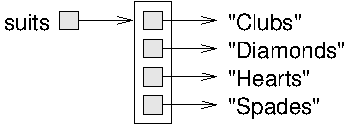
\includegraphics{figs/stringarray.pdf}

\index{state diagram}
\index{reference}
\index{String!reference to}

The elements of the array are {\em references} to the {\tt String}s,
rather than {\tt String}s themselves.

Now we need another array of {\tt String}s to decode the ranks:

\begin{code}
    String[] ranks = { "narf", "Ace", "2", "3", "4", "5", "6",
               "7", "8", "9", "10", "Jack", "Queen", "King" };
\end{code}

The reason for the {\tt "narf"} is to act as a place-keeper for the
zeroeth element of the array, which is never used (or shouldn't be).
The only valid ranks are 1--13.  To avoid this wasted element,
we could have started at 0, but the mapping is more natural if we
encode 2 as 2, and 3 as 3, etc.

Using these arrays, we can select the appropriate {\tt String}s by
using the {\tt suit} and {\tt rank} as indices.  In the method
{\tt printCard},

\begin{code}
public static void printCard(Card c) {
    String[] suits = { "Clubs", "Diamonds", "Hearts", "Spades" };
    String[] ranks = { "narf", "Ace", "2", "3", "4", "5", "6",
               "7", "8", "9", "10", "Jack", "Queen", "King" };

    System.out.println(ranks[c.rank] + " of " + suits[c.suit]);
}
\end{code}

the expression {\tt suits[c.suit]} means ``use the instance variable
{\tt suit} from the object {\tt c} as an index into the array named
{\tt suits}, and select the appropriate string.''  The output of this
code

\begin{code}
    Card card = new Card(1, 11);
    printCard(card);
\end{code}

is {\tt Jack of Diamonds}.


\section{The {\tt sameCard} method}
\label{equivalence}
\index{sameCard}

The word ``same'' is one of those things that occur in natural
language that seem perfectly clear until you give it some thought,
and then you realize there is more to it than you expected.
\index{ambiguity}
\index{natural language}
\index{language!natural}

For example, if I say ``Chris and I have the same car,'' I
mean that his car and mine are the same make and model, but they are
two different cars.  If I say ``Chris and I have the same mother,'' I
mean that his mother and mine are one person.  So the
idea of ``sameness'' is different depending on the context.

When you talk about objects, there is a similar ambiguity.  For
example, if two {\tt Card}s are the same, does that mean they
contain the same data (rank and suit), or they are actually
the same {\tt Card} object?

To see if two references refer to the same object, we use
the {\tt ==} operator.  For example:

\begin{code}
    Card card1 = new Card(1, 11);
    Card card2 = card1;

    if (card1 == card2) {
        System.out.println("card1 and card2 are identical.");
    }
\end{code}

References to
the same object are {\bf identical}.  References
to objects with same data are {\bf equivalent}.
\index{equivalent}
\index{identical}

To check equivalence, it
is common to write a method with a name like {\tt sameCard}.

\begin{code}
    public static boolean sameCard(Card c1, Card c2) {
        return(c1.suit == c2.suit && c1.rank == c2.rank);
    }
\end{code}

Here is an example that creates two objects with the same data,
and uses {\tt sameCard} to see if they are equivalent:

\begin{code}
    Card card1 = new Card(1, 11);
    Card card2 = new Card(1, 11);

    if (sameCard(card1, card2)) {
        System.out.println("card1 and card2 are equivalent.");
    }
\end{code}

If references are identical, they are also equivalent,
but if they are equivalent, they are not necessarily identical.

In this case, {\tt card1} and {\tt card2}
are equivalent but not identical, so
the state diagram looks like this:

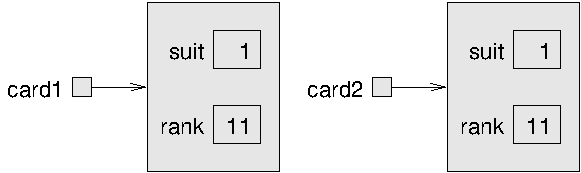
\includegraphics{figs/card.pdf}

What does it look like when
{\tt card1} and {\tt card2} are identical?
\index{aliasing}

In Section~\ref{incomparable} I said that you should not use the
{\tt ==} operator on {\tt String}s because it does not do what you
expect.  Instead of comparing the contents of the {\tt String}
(equivalence), it checks whether the two {\tt String}s are the same
object (identity).


\section{The {\tt compareCard} method}
\label{compare}
\index{compareCard}
\index{operator!conditional}
\index{conditional operator}

For primitive types, the conditional operators
compare values and determine when one is greater or less
than another.  These operators ({\tt <} and {\tt >} and the others)
don't work for object types.  For {\tt String}s Java provides
a {\tt compareTo} method.  For {\tt Card}s we have
to write our own, which we will call {\tt compareCard}.
Later, we will use this method to sort a deck of cards.

\index{ordering}
\index{complete ordering}
\index{partial ordering}

Some sets are completely ordered, which means that you can compare any
two elements and tell which is bigger.  Integers and floating-point
numbers are totally ordered.  Some sets are unordered, which means
that there is no meaningful way to say that one element is bigger than
another.  Fruits are unordered, which is why we cannot compare apples
and oranges.  In Java, the {\tt boolean} type is unordered; we cannot
say that {\tt true} is greater than {\tt false}.

The set of playing cards is partially ordered, which means that
sometimes we can compare cards and sometimes not.  For example, I know
that the 3 of Clubs is higher than the 2 of Clubs, and the 3 of
Diamonds is higher than the 3 of Clubs.  But which is better, the 3 of
Clubs or the 2 of Diamonds?  One has a higher rank, but the other has
a higher suit.
\index{comparable}

To make cards comparable, we have to decide which is more
important, rank or suit.  The choice is
arbitrary, but when you buy a new deck of cards, it comes sorted
with all the Clubs together, followed by all the Diamonds, and so on.
So let's say that suit is more important.

With that decided, we can write {\tt compareCard}.  It
takes two {\tt Card}s as parameters and returns 1 if
the first card wins, -1 if the second card wins, and 0 if
they are equivalent.

First we compare suits:

\begin{code}
    if (c1.suit > c2.suit) return 1;
    if (c1.suit < c2.suit) return -1;
\end{code}

If neither statement is true, the suits must be equal,
and we have to compare ranks:

\begin{code}
    if (c1.rank > c2.rank) return 1;
    if (c1.rank < c2.rank) return -1;
\end{code}

If neither of these is true, the ranks must be equal,
so we return {\tt 0}.


\section{Arrays of cards}
\label{cardarray}
\index{array!of object}
\index{object!array of}
\index{deck}

By now we have seen several examples of composition (the ability to
combine language features in a variety of arrangements).  One of the
first examples we saw was using a method invocation as part of an
expression.  Another example is the nested structure of statements:
you can put an {\tt if} statement within a {\tt while} loop, or within
another {\tt if} statement, etc.
\index{composition}

Having seen this pattern, and having learned about arrays and objects,
you should not be surprised to learn that you can make arrays of
objects.  And you can define objects with arrays as
instance variables; you can make arrays that contain arrays; you can
define objects that contain objects, and so on.
In the next two chapters we will see examples of these
combinations using {\tt Card} objects.

This example creates an array of 52 cards:

\begin{code}
    Card[] cards = new Card[52];
\end{code}

Here is the state diagram for this object:

\index{state diagram}

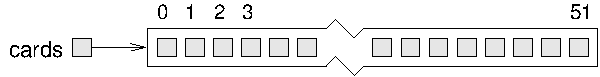
\includegraphics{figs/cardarray.pdf}

The array contains
{\em references} to objects; it does not contain the
{\tt Card} objects themselves.  The elements are
initialized to {\tt null}.  You can access the elements of
the array in the usual way:

\begin{code}
    if (cards[0] == null) {
        System.out.println("No cards yet!");
    }
\end{code}

But if you try to access the instance variables of the
non-existent {\tt Card}s, you get a {\tt NullPointerException}.
\index{exception!NullPointer}
\index{run-time error}
\index{null}

\begin{code}
    cards[0].rank;             // NullPointerException
\end{code}

But that is the correct syntax for accessing the {\tt
rank} of the ``zeroeth'' card in the deck.  This is another example of
  composition, combining the syntax for accessing an element
  of an array and an instance variable of an object.

\index{composition}
\index{loop!nested}

The easiest way to populate the deck with {\tt Card} objects
is to write nested for loops (i.e., one loop inside the body of another):

\begin{code}
    int index = 0;
    for (int suit = 0; suit <= 3; suit++) {
        for (int rank = 1; rank <= 13; rank++) {
            cards[index] = new Card(suit, rank);
            index++;
        }
    }
\end{code}

The outer loop enumerates the suits from 0 to 3.  For
each suit, the inner loop enumerates the ranks from 1
to 13.  Since the outer loop runs 4 times, and
the inner loop runs 13 times,
the body is executed is 52 times.

\index{index}

I used {\tt index} to keep track of where in the
deck the next card should go.  The following state diagram
shows what the deck looks like after the first two cards
have been allocated:

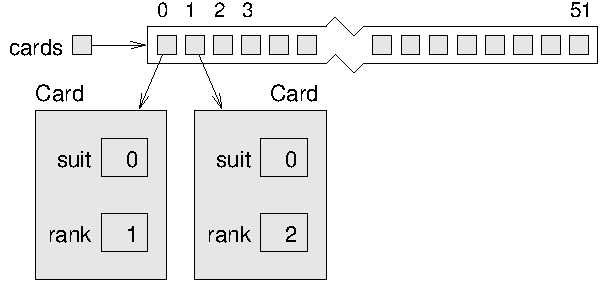
\includegraphics{figs/cardarray2.pdf}


\section{The {\tt printDeck} method}
\label{printdeck}
\index{printDeck}
\index{print!array of Cards}

When you work with arrays, it is convenient to have
a method that prints the contents.  We have
seen the pattern for traversing an array several times, so the
following method should be familiar:

\begin{code}
    public static void printDeck(Card[] cards) {
        for (int i = 0; i < cards.length; i++) {
            printCard(cards[i]);
        }
    }
\end{code}

Since {\tt cards} has type {\tt Card[]}, an element of {\tt cards}
has type {\tt Card}.  So {\tt cards[i]} is a legal argument
for {\tt printCard}.


\section{Searching}
\label{findcard}
\index{searching}
\index{findCard}

The next method I'll write is {\tt findCard}, which searches
an array of {\tt Card}s to see whether it contains a certain
card.  This method
gives me a chance to demonstrate two algorithms:
{\bf linear search} and {\bf bisection search}.
\index{linear search}
\index{bisection search}
\index{traverse}
\index{loop!search}

Linear search is pretty obvious; we traverse
the deck and compare each card to the one we are looking for.  If we
find it we return the index where the card appears.  If it is not in
the deck, we return -1.

\begin{code}
public static int findCard(Card[] cards, Card card) {
    for (int i = 0; i< cards.length; i++) {
        if (sameCard(cards[i], card)) {
            return i;
        }
    }
    return -1;
}
\end{code}

The arguments of {\tt findCard} are {\tt card} and {\tt cards}.
It might seem odd to have a variable with the same name as a type (the
{\tt card} variable has type {\tt Card}).  We can tell the difference
because the variable begins with a lower-case letter.

\index{statement!return}
\index{return!inside loop}

The method returns as soon as it discovers
the card, which means that we do not have to traverse the entire
deck if we find the card we are looking for.  If we get to the end
of the loop, we know the card is not in the deck.

If the cards in the deck are not in order, there is no way to search
faster than this.  We have to look at every card because
otherwise we can't be certain the card we want is not
there.

\index{bisection search}

But when you look for a word in a dictionary, you don't search
linearly through every word, because the words are in
alphabetical order.  As a result, you probably use an algorithm
similar to a bisection search:

\begin {enumerate}

\item Start in the middle somewhere.

\item Choose a word on the page and compare it to the word you
are looking for.

\item If you find the word you are looking for, stop.

\item If the word you are looking for comes after the word on
the page, flip to somewhere later in the dictionary and go to
step 2.

\item If the word you are looking for comes before the word on
the page, flip to somewhere earlier in the dictionary and go to
step 2.

\end {enumerate}

If you ever get to the point where there are two adjacent words on the
page and your word comes between them, you can conclude that your word
is not in the dictionary.

Getting back to the deck of cards, if we know the cards are in order,
we can write a faster version of {\tt findCard}.  The best way to
write a bisection search is with a recursive method, because bisection
is naturally recursive.  \index{findBisect}

The trick is to write a method called {\tt findBisect} that takes
two indices as parameters, {\tt low} and {\tt high}, indicating the
segment of the array that should be searched (including both
{\tt low} and {\tt high}).

\begin{enumerate}

\item To search the array, choose an index between {\tt low} and {\tt
high} (call it {\tt mid}) and compare it to the card you are looking
for.

\item If you found it, stop.

\item If the card at {\tt mid} is higher than your card, search
the range from {\tt low} to {\tt mid-1}.

\item If the card at {\tt mid} is lower than your card, search
the range from {\tt mid+1} to {\tt high}.

\end{enumerate}

Steps 3 and 4 look suspiciously like recursive invocations.  Here's
what this looks like translated into Java code:

\begin{code}
public static int findBisect(Card[] cards, Card card, int low, int high) {
    // TODO: need a base case
    int mid = (high + low) / 2;
    int comp = compareCard(cards[mid], card);

    if (comp == 0) {
        return mid;
    } else if (comp > 0) {
        return findBisect(cards, card, low, mid-1);
    } else {
        return findBisect(cards, card, mid+1, high);
    }
}
\end{code}

This code contains the kernel of a bisection search, but it
is still missing an important piece, which is why I added a TODO comment.
%
As written, the method recurses forever
if the card is not in the deck.  We
need a base case to handle this condition.
\index{recursion}

If {\tt high} is less than {\tt low},
there are no cards between them,
see we conclude that the card is not in the deck.
If we handle that case, the method works correctly:

\begin{code}
public static int findBisect(Card[] cards, Card card, int low, int high) {
    System.out.println(low + ", " + high);

    if (high < low) return -1;

    int mid = (high + low) / 2;
    int comp = compareCard(cards[mid], card);

    if (comp == 0) {
        return mid;
    } else if (comp > 0) {
        return findBisect(cards, card, low, mid-1);
    } else {
        return findBisect(cards, card, mid+1, high);
    }
}
\end{code}

I added a print statement so I can follow
the sequence of recursive invocations.  I tried out the
following code:

\begin{code}
    Card card1 = new Card(1, 11);
    System.out.println(findBisect(cards, card1, 0, 51));
\end{code}

And got the following output:

\begin{stdout}
0, 51
0, 24
13, 24
19, 24
22, 24
23
\end{stdout}

Then I made up a card that is not in the deck (the 15 of Diamonds),
and tried to find it.  I got the following:

\begin{stdout}
0, 51
0, 24
13, 24
13, 17
13, 14
13, 12
-1
\end{stdout}

These tests don't prove that this program is correct.  In fact, no
amount of testing can prove that a program is correct.  On the other
hand, by looking at a few cases and examining the code, you might be
able to convince yourself.
\index{testing}
\index{correctness}

The number of recursive invocations is typically 6 or 7,
so we only invoke {\tt compareCard} 6 or 7 times,
compared to up to 52 times if we did a linear search.  In general,
bisection is much faster than a linear search, and even more so for
large arrays.

Two common errors in recursive programs are forgetting to include a
base case and writing the recursive call so that the base case is never
reached.  Either error causes infinite recursion,
which throws a {\tt StackOverflowException}.
(Think of a stack diagram for a recursive method that never ends.)
\index{recursion!infinite}
\index{infinite recursion}
\index{exception!StackOverflow}


\section{Decks and subdecks}
\index{deck}
\index{subdeck}

\index{prototype}
Here is the prototype (see Section~\ref{documentation}) of {\tt findBisect}:

\begin{code}
public static int findBisect(Card[] deck, Card card, int low, int high)
\end{code}

\index{parameter!abstract}
\index{abstract parameter}

We can think of {\tt cards}, {\tt low}, and {\tt high}
as a single parameter that specifies a {\bf subdeck}.
This way of thinking is common, and is sometimes referred
to as an {\bf abstract parameter}.  What I mean by ``abstract'' is
something that is not literally part of the program text, but which
describes the function of the program at a higher level.

For example, when you invoke a method and pass an array and the bounds
{\tt low} and {\tt high}, there is nothing that prevents the invoked
method from accessing parts of the array that are out of bounds.  So
you are not literally sending a subset of the deck; you are really
sending the whole deck.  But as long as the recipient plays by the
rules, it makes sense to think of it abstractly as a subdeck.

This kind of thinking, in which a program takes on meaning beyond what
is literally encoded, is an important part of thinking like a computer
scientist.  The word ``abstract'' gets used so often and in so many
contexts that it comes to lose its meaning.  Nevertheless, {\bf abstraction}
is a central idea in computer science (and many other fields).
\index{abstraction}

A more general definition of ``abstraction'' is ``The process of
modeling a complex system with a simplified description to
suppress unnecessary details while capturing relevant behavior.''


\section{Glossary}

\begin{description}

\item[encode:]  To represent one set of values using another
set of values, by constructing a mapping between them.

\item[identity:]  Equality of references.  Two
references that point to the same object in memory.

\item[equivalence:]  Equality of values.  Two references
that point to objects that contain the same data.

\item[abstract parameter:]  A set of parameters that act together
as a single parameter.

\item[abstraction:]  The process of interpreting a program
(or anything else) at a higher level than what is literally
represented by the code.

\index{encode}
\index{identity}
\index{equivalence}
\index{abstract parameter}
\index{abstraction}

\end{description}



\section{Exercises}

\begin{exercise}
Encapsulate the code in Section~\ref{compare} in a method.
Then modify it so that aces are ranked higher than Kings.
\end{exercise}


\begin{exercise}
Encapsulate the deck-building code of Section~\ref{cardarray} in a method called
{\tt makeDeck} that takes no parameters and returns a
fully-populated array of {\tt Card}s.
\end{exercise}


\begin{exercise}
In Blackjack the object of the game is to get a collection of cards
with a score of 21.  The score for a hand is the sum of scores for all
cards.  The score for an aces is 1, for all face cards is ten, and
for all other cards the score is the same as the rank.  Example: the
hand (Ace, 10, Jack, 3) has a total score of 1 + 10 + 10 + 3 = 24.

Write a method called {\tt handScore} that takes an array of cards as
an argument and that returns the total score.
\end{exercise}


\begin{exercise}
In Poker a ``flush'' is a hand that contains five
or more cards of the same suit.  A hand can contain any number of cards.

\begin{enumerate}

\item Write a method called {\tt suitHist} that takes an array of Cards as a
parameter and that returns a histogram of the suits in the hand.
Your solution should only traverse the array once.

\item Write a method called {\tt hasFlush} that takes an array of Cards as a
parameter and that returns {\tt true} if the hand contains a flush,
and {\tt false} otherwise.

\end{enumerate}

\end{exercise}


\begin{exercise}
Working with cards is more interesting if you can display them on
the screen.  If you haven't played with the graphics examples in
Appendix~\ref{graphics}, you might want to do that now.

First download
\url{http://thinkapjava.com/code/CardTable.java}
and
\url{http://thinkapjava.com/code/cardset.zip} into the same folder.
Then unzip {\tt cardset.zip}, which contains a {\tt cardset-oxymoron}
subfolder with all the card images. (Note the variable {\tt cardset}
in {\tt CardTable.main} is the name of this folder.)
Run {\tt CardTable.java} and you
should see images of a pack of cards laid out on a green table.

You can use this class as a starting place to implement your own
card games.
\end{exercise}

% TODO from Leslie Klein:
% Need more descriptive text on how to modify CardTable.java so that it can find the gif files that are extracted from cardset.zip.
% If CardTable.java and all the .gif files are in the same package, and I run CardTable, I just get a green table, without the cards.
% Need text on how to set the variable cardset: the String name of the folder that contains the card images.
%-----
% Create a folder under your project called “images”. Put all the .gif files from cardset.zip into this folder.
% Make the following change in main(String[] args): change value of cardset to the name of the folder containing the images. For example,
% cardset = "images";
% Now when main() calls CardTable(cardset), CardTable can find all the gif files.
